\documentclass{article}

% if you need to pass options to natbib, use, e.g.:
%     \PassOptionsToPackage{numbers, compress}{natbib}
% before loading neurips_2021

% ready for submission
\usepackage[preprint, nonatbib]{neurips_2021}



\RequirePackage[strict=false]{csquotes}
\RequirePackage[abbreviate=false,backend=biber,language=english,sorting=none]{biblatex}
\renewcommand*{\bibfont}{\small}
\DeclareFieldFormat[misc]{title}{#1}

% lastseen date
\DeclareFieldFormat{urldate}{%
  (\bibstring{urlseen}:\addspace\thefield{urlyear}\adddot\addspace
  \mkbibmonth{\thefield{urlmonth}}\addspace\thefield{urlday}\adddot)}
  
\bibliography{bibliography}


% to compile a preprint version, e.g., for submission to arXiv, add add the
% [preprint] option:
%     \usepackage[preprint]{neurips_2021}

% to compile a camera-ready version, add the [final] option, e.g.:
%     \usepackage[final]{neurips_2021}

% to avoid loading the natbib package, add option nonatbib:
%    \usepackage[nonatbib]{neurips_2021}

\usepackage[utf8]{inputenc} % allow utf-8 input
\usepackage[T1]{fontenc}    % use 8-bit T1 fonts
\usepackage[colorlinks=true]{hyperref}       % hyperlinks
\usepackage{url}            % simple URL typesetting
\usepackage{booktabs}       % professional-quality tables
\usepackage{amsfonts}       % blackboard math symbols
\usepackage{nicefrac}       % compact symbols for 1/2, etc.
\usepackage{microtype}      % microtypography
\usepackage{xcolor}         % colors
\usepackage{graphicx}

\title{Minorities' results on the Romanian Baccalaureate}

% The \author macro works with any number of authors. There are two commands
% used to separate the names and addresses of multiple authors: \And and \AND.
%
% Using \And between authors leaves it to LaTeX to determine where to break the
% lines. Using \AND forces a line break at that point. So, if LaTeX puts 3 of 4
% authors names on the first line, and the last on the second line, try using
% \AND instead of \And before the third author name.


\author{%
  Orsolya-Renáta Szőcs\\
  Matriculation nr. 6158974\\
%   \texttt{orsolya.szocs@student.uni-tuebingen.de} \\
  \And
  Alpár Cseke\\
  Matriculation nr. 6159070\\
%   \texttt{alpar.cseke@student.uni-tuebingen.de} \\
  \AND
  \texttt{\{orsolya.szocs, alpar.cseke\}@student.uni-tuebingen.de}\\
    \texttt{\href{https://github.com/alparius/bac-stat}{https://github.com/alparius/bac-stat}}\\
}

\begin{document}

\maketitle

\begin{abstract}
    The topic of the Romanian Baccalaureate (secondary school graduation exam) instigates several assumptions regarding the difference between the results of the country's ethnolinguistic groups and that of the main population. After having scraped the last few years' results, our goal is to discuss and visualise different aspects of the gathered data to find out whether the common beliefs have a basis, and to get a better understanding of the potential underlying issues.

\end{abstract}


\section{Introduction}

\subsection{The Romanian Baccalaureate}

The Romanian Baccalaureate \cite{bac} is the exam taken by students in Romania when they graduate high school. For the most part, the baccalaureate consists of three written exams. Each written exam is graded on a scale of 1 to 10 with 10 being the best possible grade. For students to pass the exam as a whole they need to obtain a minimum of 5 on each written module and a final average of at least 6.

Romanian language and literature is one of the three written modules. This exam has to be taken by every exam participant. Moreover, each student must take a mandatory and an elective exam based on their class's study profile. In addition to these three exams, many students who belong to an ethnic minority group are also studying their native language and literature, thus must take a fourth exam in this subject.

\subsection{Minorities of Romania}
\label{ssec:min}

Romania is home to several ethnolinguistic groups who can study their native language and literature in school. The most prevalent minority group in Romania are the Hungarians with 6.3\% of the population, according to the country's last census in 2011 \cite{census}. Other linguistic minorities include the Ukrainian (0.24\%), German (0.13\%) and Turkish (0.13\%) groups.

% For the purposes of this paper, those studying one of the minority languages are treated as a single group because they all have four exams instead of three. In addition, as the children studying in these classes generally have a native language that is not Romanian, they commonly have worse knowledge of Romanian.


\subsection{Motivation}
\label{ssec:motiv}

There are several assumptions that people in Romania hold about the results of the minority groups on the baccalaureate. Some of these suppositions are the following:

\begin{itemize}
\setlength\itemsep{0em}
  \item The pupils belonging to minority groups receive worse final grades and in particular, worse grades in Romanian language and literature. The general argument for the first part of this presumption is that since the minorities need to take an additional exam, they have less time to prepare. On the other hand, people claim that as Romanian is not the native language of the minority groups, they likely have lower grades in this subject.
  \item Better minority students are less affected by their lack of Romanian linguistic knowledge on the Romanian literature exam.
  \item Students who are part of a minority have a worse chance of successfully increasing their Romanian literature grade through the grade appeal process as they get penalised for their grammatical errors that are specific to non-native Romanian speakers.
\end{itemize}

It is worth bearing in mind that these suppositions merely rely on anecdotes and personal observations. Our goal is to challenge these assumptions by utilising the available data.

%Being minority members, most of the assumptions we encountered revolved around comparisons between the main Romanian population and the different ethnolinguistic groups. Having to take a fourth exam while still getting the same full subject on the Romanian one is a recurring pain point, but the other side often argues that this mother tongue language and literature exam is too easy compared to the rest of the examination, raising the averages.

%Another widespread presupposition is that when minorities' appealed Romanian language and literature exams get sent to predominantly Romanian counties (which they very likely are), it probably gets downgraded if the person evaluating the exam recognises the pupil as a minority from their writing style.


% A list of common assumptions:
% \begin{itemize}
% \item The minorities have worse final grades because they have to study for 4 subjects instead of just 3. \emph{(Final grade distribution minority (maybe even Hungarian, German separately) vs Romanian. Final grade minority vs Romanian.}
% \item The minorities have worse scores in Romanian than the Romanians but the minorities’ native language grade raises their final grade. \emph{(PDF of minority vs Romanian grade. Romanian grade plotted against Hungarian grade or Romanian against final grade.)}
% \item The minorities have better foreign language skills.
% \item For better students, being part of the minority makes less of a difference: the Romanian grade is still high - but for worse students it makes it even worse.
% \item Students studying in science classes have better grades than those studying in humanity classes. (Only if there is space)
% \end{itemize}


\section{Methodology}

Our language of choice for manipulating the data was \emph{Python}, together with its staple data stack (i.e. \emph{pandas, numpy} and \emph{matplotlib}). The experiments themselves were carried out in \emph{Jupyter Notebook} to facilitate a step-by-step workflow and make results reproducible.


\subsection{Data Acquisition}

The underlying dataset was acquired from the official site of the examination \cite{bactable}. Only the last three years (2019, 2020, 2021) were available. Earlier results were removed from the site since those were not anonymised.

The data was scraped with the \emph{Selenium} library \cite{selenium}, which utilises a headless browser to render the target webpages using a stripped-down version of the browser's engine. Static scraping methods did not prove to be successful due to the \emph{JavaScript} code present in several of the table's cells.

The scraping itself turned out to be times of magnitudes slower than initially expected, therefore the script was extended for parallel execution: to save data to files in smaller batches and to always check for already collected chunks by other processes.

Furthermore, it must be noted that the scraping process abode by the webpage's \emph{robots.txt} ruleset: the resource was not disallowed and we respected the 10 second request frequency (although the long running time was also a limitation of our code). The total process involved not more than 40 000 URL requests spread across multiple days.

\section{Experiments and results}

In this section we examine the results of the baccalaureates held in 2019, 2020 and 2021. Since the difficulty level of the individual exam modules varies each year, we believe that through combining the results from the three years we obtain data that is more representative of the general baccalaureate exam.

\begin{table}[!b]
  \caption{Number of participants at the Romanian Baccalaureate}
  \label{group-size}
  \centering
  \begin{tabular}{l|llll}
    \toprule
    Student group & Size (2019) & Size (2020) & Size (2021) & Total size \\
    \midrule
    \textit{R} & 121 693 & 140 315 & 120 472 & 382 480 \\
    \textit{M} & 6 826 & 7 351 & 6 381  & 21 528 \\
    \bottomrule
  \end{tabular}
\end{table}

\begin{table}[!b]
  \caption{Average final grades at the Romanian Baccalaureate}
  \label{group-average}
  \centering
  \begin{tabular}{l|llll}
    \toprule
    Student group & Average (2019) & Average (2020) & Average (2021) & Total average \\
    \midrule
    \textit{R} & 7.007 & 6.820 & 7.030 & 6.946 \\
    \textit{M} & 6.868 & 6.994 & 7.013 & 6.958 \\
    \bottomrule
  \end{tabular}
\end{table}

We denote the group of students who had to take only three written exams as \textit{R}. Those studying one of the minority languages are treated as a single group \textit{M} because they share the common trait of having four exams instead of three. It must be noted that their actual distribution is similar to the one presented in subsection \ref{ssec:min}, with Hungarians accumulating to 5.3\% of exam participants and all of the other minorities totalling up to 0.7\%. 

Table \ref{group-size} shows the number of the students not disqualified from any of the exams (i.e. with valid grades). Table \ref{group-average} displays the average final grades of the two groups in each year. Although we can not tell whether or not the grades of \textit{M} would be greater if they only had to take three exams, we observe that the difference between the average final grades of \textit{R} and \textit{M} is very small. Therefore, based on these three years' data, \textit{M} does not seem to be at disadvantage when considering only the final grades.
 
 
\begin{figure}[!b]
    \centering
    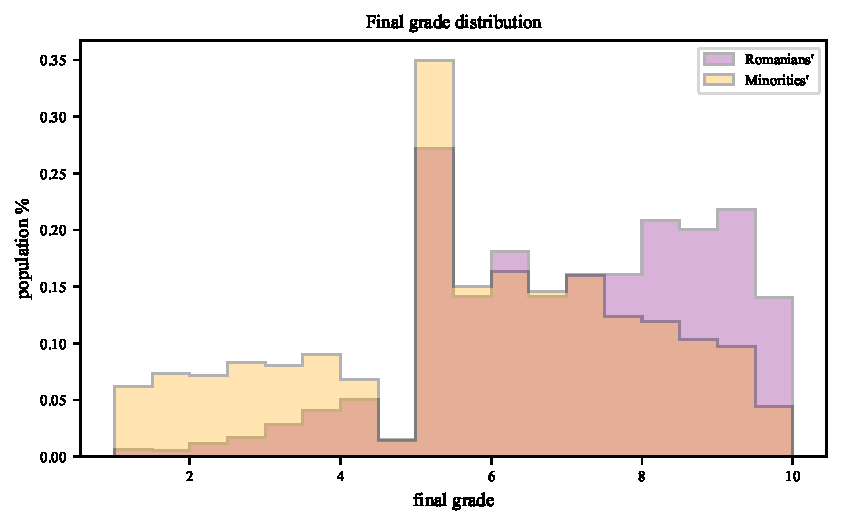
\includegraphics[width=14cm]{plots/exp4_grade_distrib.pdf}
    \caption{Distribution of the Romanian language and literature grades}
    \label{fig:ro-distr}
\end{figure}

\begin{figure}[!b]
    \centering
    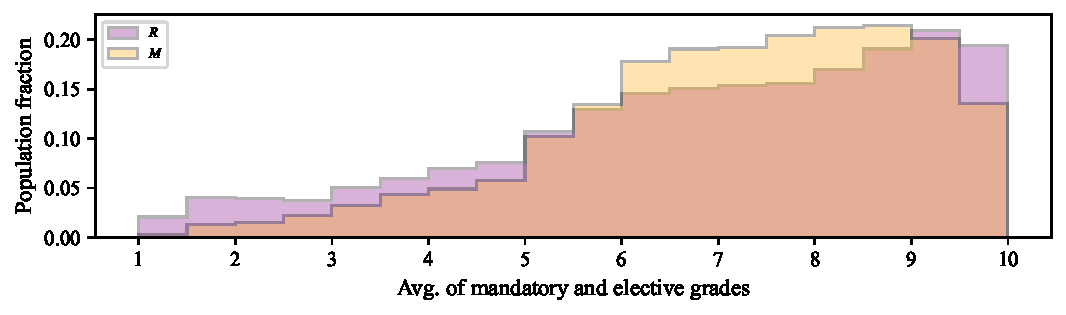
\includegraphics[width=14cm]{plots/exp4_grade_distrib_spec.pdf}
    \caption{Distribution of the average of the mandatory and elective subject grades}
    \label{fig:subj-distr}
\end{figure}


The distribution of the final grades in Romanian language and literature is shown in Figure \ref{fig:ro-distr}. A notable aspect of this distribution is that there are relatively few grades between 4 and 5 and many grades between 5 and 5.5. A probable explanation for this is that teachers correcting the exam might be less strict when the student's grade would otherwise fall right below the minimum passing grade.

The plot shows that group \textit{M} achieves worse grades than \textit{R} on this particular exam. The average grade in this subject for \textit{R} is 7.060, while for \textit{M} it is 5.744. Thus, on average, group \textit{R} achieves a grade greater by 1.316, which equates to a difference of 14.62\%.

% If the Romanian literature grades contain such a big discrepancy between \textit{M} and \textit{R}, yet the average final grades are close, something must account for this difference. \textit{M}'s average grade in their mother tongue language and literature exam is 7.630.

It is worth comparing \textit{M}'s grade in their native language and literature to \textit{R}'s Romanian literature grade. \textit{M}'s average native language grade is 7.630, which is greater by 0.570 than the average Romanian grade of \textit{R} and by 1.886 than the average Romanian grade of \textit{M}. Yet, this greater native literature grade does not fully account for how group \textit{M} makes up for their lesser Romanian literature grades to have an almost even average final grade. 

Figure \ref{fig:subj-distr} shows that the rest of the discrepancy between the two groups lies in their specialisation-specific grades. Proportionally to their sizes, \textit{M} achieves considerably more grades in the 6 to 9 grade buckets, summing up to a 0.294 higher average grade in the two specialization-specific exams. Specifically, \textit{R}'s average is 6.888 as opposed to \textit{M}'s 7.182.

This difference is not negligible, since the mandatory and elective exams of the specialisation should have very little to do with the participants' native languages. The phenomenon could have several different explanations: minority schools might better prepare students for their study profile exams, or the minority exam graders could be less strict.


\begin{figure}
    \centering
    \begin{minipage}[t]{0.49\textwidth}
        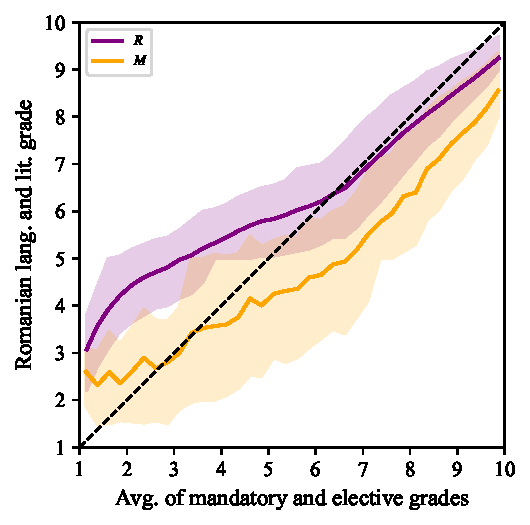
\includegraphics[width=7cm]{plots/exp1_grade_plot.pdf}
        \caption{Expected Romanian language and literature grades given the average of the specialisation's mandatory and elective grades}
        \label{fig:ro-vs-subj}
    \end{minipage}
    \hfill
    \begin{minipage}[t]{0.49\textwidth}
        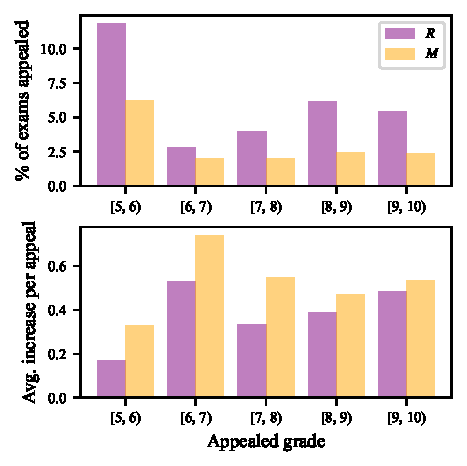
\includegraphics[width=7cm]{plots/exp6_appeal_ro.pdf}
        \caption{Percentage of students in each grade group submitting a grade appeal for their Romanian lang. and lit. exam (top). Average increase in grade after the appeal (bottom)}
        \label{fig:appeal}
    \end{minipage}
\end{figure}



Figure \ref{fig:ro-vs-subj} is achieved by separating the examinees into 36 groups based on the average of the grades specific to their study profiles and computing the average Romanian language grade for each group. Additionally, the plot also shows the area bounded by the 25\textsuperscript{th} and 75\textsuperscript{th} percentiles.

We can observe that in the case of both \textit{M} and \textit{R} better specialisation grades generally lead to better grades on the Romanian exam. Supporting the assumption that better \textit{M} students are at a lesser disadvantage at the Romanian literature exam, we can notice that the difference does tighten between the Romanian grades of \textit{M} and \textit{R} when their average specialisation grade is above 8.

% Yet, the minority native grade is higher than the average Ro grade. Again, can use Cohen's d effect size.

% Language skills

% Specialisations

Our last assumption underlined in subsection \ref{ssec:motiv} is regarding the improper treatment of Romanian language and literature grade appeals submitted by \textit{M} members. What the top part of Figure \ref{fig:appeal} reveals is that only a considerably smaller percentage of \textit{M} requests a grade appeal in this exam module. Presumably, they require more confidence in a successful re-evaluation. This is a feasible explanation to the bottom plot of the figure, namely that \textit{M} receives on average a higher increase in their final grade from their grade appeals.





\section{Conclusion}

The work on the subject is far from conclusive. Having not done actual hypothesis testing or causal inference, we can not claim any quantifiable results over our initial assumptions. More so, this paper is intended as a discussion starter in the grand topic of examination fairness across the diverse minority groups of today's countries.  



%Having not done actual statistical tests on the data, we cannot confidently claim any quantifiable result over our initial assumptions.

% conclusions: impact, future work, limitations



\printbibliography

\end{document}
